%----------------------------------------------------%
%                    INTRODUCCION                    %
%----------------------------------------------------%

\pagestyle{fancy}

\chapter{Introducción}
\label{introduccion}

Desde Aristóteles y su libro Segundos Analíticos hasta Galileo, padre de la ciencia moderna, muchos adalides del conocimiento han proclamado que un método de investigación basado en lo empírico y en la medición, sujeto a los principios específicos de las pruebas de razonamiento es el camino para alcanzar la verdad.\\

Hoy en día, época en la que los avances tecnológico han posibilitado observar y medir de forma exhaustiva un gran abanico de fenómenos, la ingente cantidad de datos que se genera en el proceso es, a veces, intratable por medio de las tecnologías convencionales, y por ende, imposible extraer conocimiento de ellos. El problema, lejos de atenuarse, se acrecienta con el paso del tiempo, ya que, estudios como el realizado por McKinsey Global Institute (MGI) estiman que el volumen de datos que se genera está creciendo un 40\% cada año y auguran  que entre 2009 y 2020 se verá multiplicado por 44[1].\\

Por ello, en los últimos años ha irrumpido la necesidad de encontrar metodologías y herramientas que permitan procesar y extraer el conocimiento que atesora el torrente de información en la cual se encuentra envuelta la sociedad, dando como resultado el nacimiento del Big Data.\\

El mundo empresarial, por su parte, no se ha mantenido al margen de esta gran revolución. Conscientes de los beneficios que les puede reportar en diferentes aspectos como en el análisis de mercado y calidad de los servicios que ofertan, la gran mayoría de las empresas se han interesado en el Big Data. De un estudio realizado entre los altos ejecutivos de las firmas que lideran el Wall Street se desprende que el 96\% tiene planeadas ciertas iniciativas relacionadas con el Big Data, y el 80\% tiene finalizada alguna[2]. 

\section{Contexto}
 
Datik Información Inteligente S.L. es una empresa tecnológica perteneciente al Grupo Irizar  que desarrolla soluciones ITS destinadas a la gestión del trasporte, tanto ferroviario como por carretera y movilidad ciudadana.\\

Uno de los productos estrella de la entidad es el denominado iPanel, concentrador de  información que ofrece al operador de transporte servicios de valor añadido en la gestión de la información generada por su flota. El funcionamiento de este servicio se puede resumir mediante la Figura \ref{fig:ipanel}:\\

\begin{figure}[h]
	\centering
	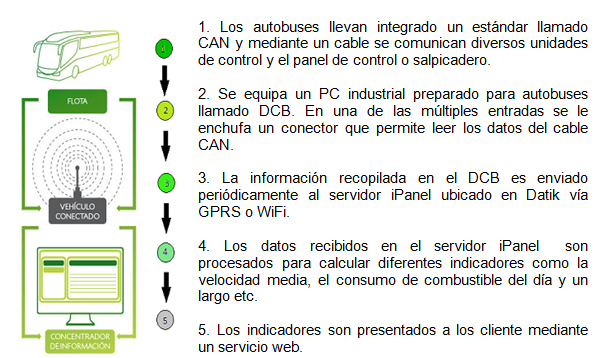
\includegraphics[width=1\textwidth]{Ilustraciones/ipanel_infraesctructure.png}
	\caption{Funcionamiento resumido de iPanel}
	\label{fig:ipanel}
\end{figure}

El incesante aumento en el número de vehículos equipados genera un crecimiento exponencial de los elementos que se han de almacenar y procesar en una base de datos MySQL. Aunque el volumen de datos con el que se trabaja hoy en día no supone riesgo alguno para el funcionamiento del servicio, Datik tiene identificados varios escenarios en los que esto podría cambiar, dando pie al afloramiento de graves problemas.\\

El primero de todos, es el tiempo necesario para realizar el cálculo de los indicadores. Se trata de un proceso ejecutado una vez al día que atendiendo los datos recopilados en las últimas 24 hora vuelve a calcular todos los indicadores de iPanel. Ello implica realizar operaciones aritméticas sobre diferentes campos como la velocidad y el consumo de combustible y agrupar los resultados por cliente, flota, vehículo o un espacio temporal. Actualmente, se necesitan varias horas para finalizar la computación, pero, debido al aumento de los datos a tratar, es posible que en un futuro existan graves dificultades para realizar el calculo en menos de 24 horas, invalidando así la funcionalidad de ofrecer los indicadores del último día.\\

Otro de los problemas, intrínseco al uso de una base de datos centralizada, es el operar sobre un único punto de fallo. Debido a que la mayoría de procesos pasan por dicho punto, existe un alto riesgo de sufrir el denominado efecto dominó, esto es, que la caída provocada por un servicio acarree la del resto. Actualmente, Datik dispone un servidor de réplica capacitado para suplir al primario en caso de que ocurra algo así. No obstante, esta práctica condenar una máquina al ostracismo ya que sus recursos quedan desaprovechados en el 99,95\% del tiempo.\\

EL último, es la corrupción de datos. Este fenómeno puede suceder (y sucede) debido a un bug, fallo de almacenamiento inesperado, o una caída de MySQL cuando el resultado del checksum de una página es diferente al esperado. Como resultado, podría comprometer seriamente la información que Datik ofrece a sus clientes mediante la aplicación web.\\

\section{Propuesta}

Para solventar los problemas que Datik prevé, se propone implantar las tecnologías Apache Cassandra y Apache Spark en la empresa y migrar tanto las tablas como los procesos que son parte en el cálculo de los indicadores.\\


Apache Cassandra es una base de datos distribuida no-sql. Gracias a naturaleza distribuida ayuda a resolver, 






Diseñar un plan de migración que defina aspectos tales como: 

\begin{itemize}
	\item Listado de las tablas MySQL que deben ser migradas a Cassandra priorizando las que más rápido crecen y mayor número de consultas intensivas reciben. Por ejemplo, las tablas que contienen la información para el calculo de los indicadores.
	\item Listado tablas "frontera"
	\item Ver por cada ejercicio su estado de realización: quiénes lo han terminado, quiénes tienen duda y quiénes no han respondido nada.
	\item Editar cualquier detalle de un ejercicio en cualquier momento.
	\item Valorar la realización de un ejercicio a un alumno concreto.
\end{itemize}

el traspaso de las tablas MySQL que mayor velocidad crecen  y mayor número de consultas pesadas reciban a estas nuevas tecnologías. empezando por las que tienen estrecha realción con el calculo de indicadores, ya que, como se ha indicado con anterioridad, es  

Por su parte, Apache Cassandra

Por Apache Spark por otra,

Debido a la falta de datos se ha utilizado un dataset publico para emular las condiciones de futuro con las que se va a encontrar datik

\section{Organización del documento}

En esta memoria se ha documentado  el desarrollo de la herramienta \textbf{\textit{exerClick}}, dentro del Trabajo de Fin de Grado (TFG) del autor. En el documento se describe la propuesta, la planificación y gestión que esta lleva consigo, la implementación llevada a cabo y las conclusiones finales.\\

En este primer capítulo se ha introducido el problema a resolver y se ha explicado la propuesta presentada en este proyecto.\\

En el capítulo 2 se presenta el Documento de Objetivos de Proyecto (DOP). Este recoge el alcance y las fases y tareas del proyecto, el análisis de riesgos y el análisis de factibilidad.\\

Una vez en el capítulo 3 se explica la gestión llevada a cabo durante el proyecto. Se presentan las metodologías utilizadas: Metodologías Ágiles e InterMod (adaptada a las necesidades de este proyecto). A continuación se detallan cada una de las iteraciones llevadas a cabo (como parte de la metodología InterMod): duración, objetivos y tareas realizadas. Al final del capítulo se muestra la documentación asociada a las iteraciones y los objetivos, además del seguimiento de tiempo realizado.\\

A continuación, en el capítulo 4 se detalla el análisis de requisitos. Primero se detallan los requisitos no-funcionales y luego los funcionales (prototipos en papel llevados a cabo durante las primeras iteraciones que dan una visión global del proyecto).\\

En el capítulo 5 se explica el diseño e implementación llevados a cabo. Se comienza mostrando la estructura de documentos del proyecto, luego el diseño realizado en base al análisis de requisitos del capítulo 4 y finalmente una visión general de la implementación de la lógica de negocio.\\

Para finalizar, en el capítulo 6 se presentan las conclusiones, líneas futuras para el proyecto y las lecciones aprendidas.\\

Fuera de la estructura general de la memoria, tenemos la bibliografia y los apéndices. En estos últimos tenemos las actas de reuniones, las actas de pruebas y la vista de relaciones de la base de datos (de la parte utilizada o creada específicamente para el proyecto).\\